\subsection{Nutrient-Mediated Regulation of Proteomic Composition and Growth Rate}
To react to changes in nutrient conditions, bacteria rely on the synthesis or
degradation of secondary-messenger molecules  like (p)ppGpp, which cause global
changes in transcriptional and translational activity. In \textit{E. coli},
amino acid starvation causes the accumulation of de-acylated tRNAs at the
ribosome's A-site and leads to a strong increase in (p)ppGpp synthesis activity
by the enzyme RelA \citep{hauryliuk2015}. Cells also accumulate (p)ppGpp  during
steady-state growth in poorer growth conditions, which leads to a decrease in
the fraction of actively translating ribosomes, $f_a$  (with $f_a \approx 0.5$
at a growth rate of $\approx$ 0.3 hr$^{-1}$; \FIG{ribosome_limit}(C) - inset).

Furthermore, (p)ppGpp can inhibit the initiation of DNA replication by mediating
a change in transcriptional activity and the supercoiling state of the origin of
replication \citep{kraemer2019}. These observations all raise the possibility
that it is through (p)ppGpp that cells mediate the growth-rate dependent changes
in $\langle$\# ori$\rangle$, cell size, and ribosomal abundance and activity
\citep{zhu2019, Buke2020}. Indeed, recent work in a (p)ppGpp deficient strain of
\textit{E. coli} found that cells exhibited a high ratio in the number of
origins of replication to the number of termini, and cell sizes that were more
consistent with a fast growth state where (p)ppGpp levels are normally low
\citep{fernandezcoll2020}.

As we have seen, cell size, total proteomic content, and the number of ribosomes
are all interconnected and influence the achievable growth rate. In this final
section, we consider this interconnection by formulating a minimal model of
growth rate control. We use it to quantitatively show how tuning these
parameters help cells maximize their growth rate for a particular environment.

% The drastic changes observed in cell size, proteomic composition, and
% ribosome abundance across different growth conditions suggests a hypothesis
% that each parameter is being tuned to better match the cell's biosynthetic
% capacity to the specific environment.


\subsubsection{Ribosomal Elongation Rate and Cellular Growth Rate are Linked by
Amino Acid Scarcity}
Here we consider a mode of regulation in which the rate of peptide elongation
$r_t$ depends only on the availability of amino acids (and, therefore, also
amino-acyl tRNAs). It is through the elongation rate $r_t$ that we assume cells
adjust their ribosomal content ($R$, $\Phi_R$) according to nutrient
availability and for simplicity, do not explicitly model changes in  $\langle$\#
ori$\rangle$ or regulation by (p)ppGpp.

The rate of elongation $r_t$ will depend on how quickly the ribosomes can match
codons with their correct amino-acyl tRNA, along with the subsequent steps of
peptide bond formation and translocation. We therefore coarse-grain the steps of
elongation to two time-scales,  1) the time required to find and bind each
correct amino-acyl tRNA, and 2) the remaining steps in peptide elongation that
will not depend on the amino acid availability. The availability of amino acids
will depend on their cellular concentration, which we treat as a single
effective species, $[AA]_\text{eff}$. Under this model, other molecular players
required for translation like elongation factors and GTP are considered in
sufficient abundance, which appear to be valid assumptions given our analysis of
the proteomic data and energy production thus far. The time to translate each
codon is given by the inverse of the elongation rate $r_t$, which can be written
as,

\begin{equation}
\frac{1}{r_t} = \frac{1}{k_{on} \alpha [AA]_{\text{eff}}} + \frac{1}{r_{t}^{\text{max}}}.
\end{equation}
where we have assumed that the rate of binding by amino-acyl tRNA $k_{on}$ is
proportional to $[AA]_{\text{eff}}$ by a constant $\alpha$. The second term on
the right-hand side reflects our assumption that other steps in peptide
elongation are not rate-limiting, with a maximum elongation rate
$r_{t}^{\text{max}}$ of about 17 amino acids per second \cite{dai2016}. As the
rate of amino acid supply, denote by $r_{AA}$, varies with changing nutrient
conditions, the cell can maximize the rate of protein synthesis by tuning the
rate of amino acid consumption ($r_t \times R \times f_a$) ,
shown schematically in \FIG{elongation_rate_model}(A). This can be stated more
succinctly in terms of an effective dissociation constant, $K_D = r_{t}^{\text{max}} / \alpha k_\text{on}$, where the elongation rate $r_t$ is now given by

\begin{equation}
r_t = \frac{r_{t}^{\text{max}}}{1 + K_D/[AA]_{\text{eff}}}.
\label{eq:rt_kd_simple}
\end{equation}

Under steady-state growth, the amino acid concentration is constant
($\frac{d[AA]_\text{eff}}{dt}=0$) and will relate to the rate of amino acid
synthesis (or import, for rich media) and/or tRNA charging, as $r_{AA}$, and the
rate of consumption, $r_t\times R \times f_a$. We calculate
$[AA]_\text{eff}$ by,

\begin{equation}
   [AA]_\text{eff} = \frac{t(r_{AA} - r_t \times R \times f_a)}{V},
   \label{eq:aa_final}
\end{equation}
which allows us to then solve for $r_t$ explicitly (further described in
Appendix \ref{sec:SI_model}). Here $r_{AA}$ is in units of AA per unit time, and
$V$ reflects the volume of the cell over a time period $t$.

In \FIG{elongation_rate_model}(B), we illustrate how the elongation rate depends
on the ribosomal copy number. Here, we have considered a unit volume $V =
1$\textmu m$^3$, a unit time $t = 1$ s, a $K_D = 5$ mM (inferred from
\cite{bennett2009}), $f_a = 1$, and an arbitrarily chosen $r_{AA} = 5\times 10^6$ AA
$\cdot$ s$^{-1} \cdot$ \textmu m$^{-3}$. At low ribosome copy numbers, the
observed elongation rate is dependent primarily on the ratio of $K_D / Vr_{AA}$
[as $r_t^{\text{max}} \times R \times f_a << r_{AA}$, point (1) in
\FIG{elongation_rate_model}(B)]. As the ribosome copy number is increased such
that the amino acid supply rate and  consumption rate are nearly equal [point
(2) in \FIG{elongation_rate_model}(B)], the observed elongation rate begins to
decrease sharply. When the ribosome copy number is increased even further,
consumption at the maximum elongation rate exceeds the supply rate, yielding  a
significantly reduced elongation rate [point (3) in
\FIG{elongation_rate_model}{B)]. While the elongation rate will always be
dominated by the amino acid supply rate at sufficiently low ribosome copy
numbers, the elongation rate at larger ribosome abundances can be increased by
tuning $f_a$ such that not all ribosomes are elongating, reducing the total
consumption rate.

\begin{figure}
    \centering{
        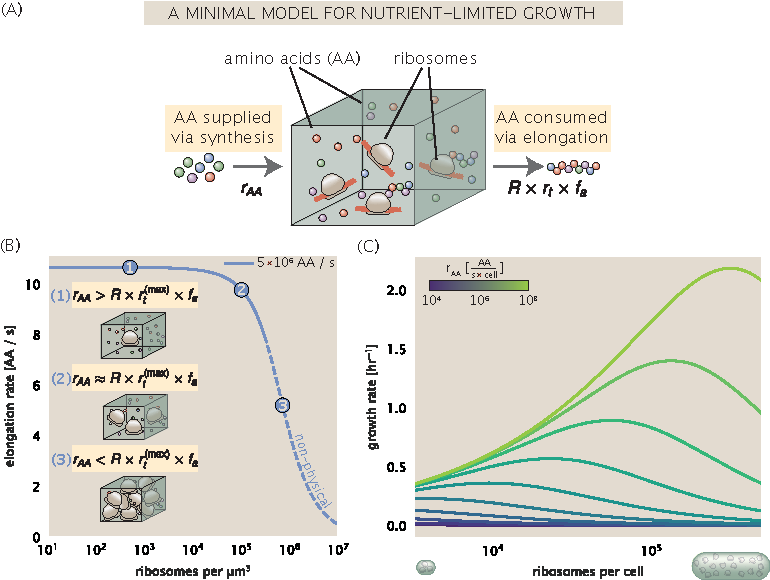
\includegraphics{main_figs/elongation_model.pdf}
        \caption{\textbf{A minimal model of growth rate control under
        nutrient limitation.} (A) We consider a unit volume of cellular material
        composed of amino acids (colored spheres) provided at a supply rate
        $r_{AA}$. These amino acids are polymerized by a pool of ribosomes
        (brown blobs) at a rate $r_t \times R \times f_a$, where $r_t$ is the
        elongation rate, $R$ is the ribosome copy number in the unit volume, and
        $f_a$ is the fraction of those ribosomes actively translating. (B) The
        observed elongation rate is plotted as a function of ribosomes in a unit
        volume \textmu m$^3$. The three points correspond to three regimes of
        ribosome copy numbers and are shown schematically on the left-hand side.
        The region of the curve shown as dashed lines represents a non-physical
        copy number, but is shown for illustrative purposes. This curve was
        generated using the parameters $r_{AA} = 5 \times 10^6$ AA / s, $K_D =
        5$ mM, and $r_t^\text{(max)} = 17.1$ AA / s. (C) The cellular growth
        rate is plotted as a function of total cellular ribosome copy number for
        different cellular amino acid supply rates, with blue and green curves
        corresponding to low and high supply rates, repsectively. As the
        ribosome copy number is increased, so too is the cell volume and total
        protein abundance. We direct the reader to the Suppemental Information
        for discussion  on the inference of the realtionship between cell
        volume, number of peptide bonds, and ribosome copy number.}
        \label{fig:elongation_rate_model}
    }
\end{figure}

\subsubsection{Optimal Growth Rate, Ribosomal Content, and Cell Size Depend on Nutrient
Availability and Metabolic Capacity.}

To relate elongation rate to growth rate, we constrain the set of parameters
based on our available proteomic measurements; namely, we restrict the values of
$R$, $N_{pep}$, and $V$ to those associated with the amalgamated proteomic data
(described in Appendix \nameref{sec:estimate_protein_per_cell}). We then consider
how changes in the nutrient conditions, through the parameter $r_{AA}$,
influence the maximum growth rate as determined by \EQ{lambda_limit}.
\FIG{elongation_rate_model}(C) shows how the observed growth rate depends on the
rate of amino acid supply $r_{AA}$ as a function of the cellular ribosome copy
number. A feature immediately apparent is the presence of a maximal growth rate
whose dependence on $R$ (and consequently, the cell size) increases with
increasing $r_{AA}$. Importantly, however, there is an optimum set of $R$,
$N_{pep}$, and $V$ that are strictly dependent on the value of $r_{AA}$.
Increasing the ribosomal concentration beyond the cell's metabolic capacity has
the adverse consequence of depleting the supply of amino acids and a concomitant
decrease in the elongation rate $r_t$ [\FIG{elongation_rate_model}(B)].

Also of note is the growth rate profiles shown for low amino acid supply rates
[purple and blue lines in \FIG{elongation_rate_model}(C)], representing growth
in nutrient-poor media. In these conditions, there no longer exists a peak in
growth, at least in the range of physiologically-relevant  ribosome copy
numbers. Instead, cells limit their pool of actively translating ribosomes  by
decreasing $f_a$ \citep{dai2016}, which would help maintain the pool of
available amino acids $[AA]_\text{eff}$ and increase the achievable elongation
rate. This observation is in agreement with the central premise of the cellular
resource allocation principle proposed by \cite{scott2010,
klumpp2009,klumpp2014} and \cite{hui2015}.
